\documentclass{acm_proc_article-sp}
\usepackage{url}
\begin{document}


%make title bold and 14 pt font (Latex default is non-bold, 16 pt)
\title{\Large \bf Social Math: A collaborative, visual host for mathematical proof trees}
\numberofauthors{4} %  in this sample file, there are a *total*
% of EIGHT authors. SIX appear on the 'first-page' (for formatting
% reasons) and the remaining two appear in the \additionalauthors section.
%
\author{
\alignauthor
Jianchi Chen\\
       \affaddr{Dept. of Electronical Engineering}\\
       \email{jchen2@caltech.edu}
\alignauthor
Ying-Yu Ho\\
       \affaddr{Dept. of Physics,}\\
       \affaddr{Mathematics, and Astronomy}\\
       \email{yingyu@caltech.edu}
\alignauthor
Tim Holland\\
       \affaddr{Dept. of Computing and}\\
       \affaddr{Mathematical Sciences}\\
       \email{th0114nd@gmail.com}
\and  % use '\and' if you need 'another row' of author names
\alignauthor 
Kexin Rong\\
       \affaddr{Dept. of Computing and}\\
      \affaddr{Mathematical Sciences}\\
      \email{krong@caltech.edu}
}

\maketitle

% Use the following at camera-ready time to suppress page numbers.
% Comment it out when you first submit the paper for review.
\thispagestyle{empty}

\subsection*{Abstract}
Mathematical proofs and theorems, and the inter-dependencies among them (edges) have the structure of a directed acyclic graph (DAG). However, in most educational processes or online mathematical libraries, theorems and proofs are typically presented in a linear fashion, which fails to connotate the theorem's inter-relationship with others, or how it is positioned in the mathematical world. Therefore, we propose a web service to better present mathematical proof trees as graphs, and allows users from all over the world to contribute to the graph, and use it for their own interest. Supposedly, the visualization should  help users both navigate through the existing mathematical library and also easily contribute new proofs to expand the reach of the proof trees. The service can serve as a stand alone online crowd sourced mathematical library, or can be incorporated into other systems as a tool to visualize logical inter-relationship. 

\keywords{proof trees, visualization, social network, education, graph} % NOT required for Proceedings

\section{Introduction}
The course of mathematical study can be frustrating. After proving one lemma after another, students can easily get caught in the details and forget about the big picture. In another case, students can learn 10 different theorems without understanding how they are related to each other.  The difficulty is caused by the lack of an intuitive ways to visualize these concepts and their relationships. If we model mathematical theorems and proofs as nodes, and their relationships as directed edges, a mathematical library is indeed a set of "proof trees" with the structure of a DAG. Acyclic is guaranteed by the fallacy of circular reasoning. 
 
We therefore created a service and web based front end that allows the entry, modification, inspection, and visualization of theorems, definitions, proofs and the dependencies between them. Dependencies include the relationship between a theorem and its proof, between a proof and its lemma, or a theorem/definition and its special case/generalization.

We have two possible choices to proceed on how to keep the DAG logically sound. The first is more of an advanced technical problem: automatic proof-logic verification, requiring highly precise statements of additions to the tree to be parsed, so that the logical statements can then be verified (or rejected) by machine. Alternatively, with a more social emphasis proofs could be stated in natural mathematical language. Under this scheme, the correctness would have to be verified by users, through a combination of moderation, reputation, and democracy.

We hope that this is a service with fruitful pedagogical applications. For example, in a class taught via the Moore Method, the service could be used as a study tool: A set of isolated definitions and theorems are given at the start of the term. Students' progress can be easily assessed from the completeness of the graph visualization. 

Alternatively, the service can be incorporated as an useful feature for other web services. The idea of a mathematical proof tree can be generalize to a knowledge graph in any field.  For sites like Wikipedia, having a graphic interface navigation to provide a map of topics to learn and modify can greatly enhance user experiences.



\section{Related Work}
Expii \cite{expii} is an extensive crowdsourced MOOC service that has  launched recently. It currently focuses on topics in Math and Physics, and provides a zoom in style visualization of the knowledge graph. When users zoom in from section "Three Big Perspectives for Calculus" for example, they can see three subsections "Algebra", "Analytic Geometry" and "Sets and Maps". Further zooming in from subsection "Sets and Maps" will lead users to sub-subsections "Set Definitions", "Special Sets" and "Functions as Maps Between Sets".

Despite being similar crowd sourced products with knowledge graph visualization, Expii and socialmath have distinct end goals. Expii aims to the biggest interactive tutor, while socialmath focuses on becoming a intuitive and comprehensive mathematical library. As a result, Expii organizes topics in a pedagogical manner while socialmath organizes according to logical dependencies. For instance, theorems in algebra and analytic geometry might not directly depend on each other, but these two topics are closed related as background knowledge to calculus. 

\section{Timeline}
\subsection{Initial Timeline}
Below is the initial project timeline we proposed at the project proposal presentation. The plan was to build a working prototype before midterm, and to add as many features as time allows afterwards.  
\begin{itemize}
\item Week 2 - 5: Basics
\begin{itemize}
\item Client-server API
\item Database API
\item Implement views and templates for browsing, editing, and adding theorems
\item Front end visualization
\end{itemize}
\item Week 6: Milestone:\\
Should have a simple working prototype, which allows adding, deleting and viewing nodes from the proof DAG
\item Week 7 - 9: Useful advanced features
\begin{itemize}
\item Search by keywords
\item User profile
\item Private graph
\item Auto-keyword-extraction
\item Suggested theorems
\end{itemize}
\end{itemize}

\subsection{Actual Timeline}
Below is a summary of our actual weekly progress based on the blogs. The front end progress was highly non-linear because we either underestimated the amount of work or overestimated the ability to stick to schedule of the person in charge. Thus most features were first implemented on the server-side, and then enhanced with Ajax. Nevertheless, we were able to implement the three most useful advanced features: keyword search, user profile and private graph. A detail description of the end product is given in the next section.
\begin{enumerate}
\item \emph{Week 1: Changing Gears}\\\\
Due to the discovery of a fairly comprehensive open source traffic simulator project, we decided to abandon the original 144 project proposal and to work, instead, on a web application that accommodates the visualization of mathematical proof tree structures. We discussed the basic application architecture, and decided to use the typical LAMP stack with a REST API and CRUD functionality. In our case the P stands for Python with Django REST framework, the M stands for SQLite, and the A could either be Apache or Amazon Web Service.\\\\
The first steps we took were similar to any team making a CRUD app: setting up the database and a method of communication between the client and server. Specifically, we determined a schema for the database and fleshed out data structures for the DAG. We also started to familiarized ourselves with the frameworks that we will be working with for the rest of the term.\\\\
On the front end side, several JavaScript frameworks quickly came to our mind:
AngularJS\cite{Google:2014:Online} and/or jQuery for DOM manipulation, Bootstrap\cite{UI:2014:Online} for style and UI components, and D3.js \cite{Bostock:2014:Online} for data visualization. These frameworks have some overlapping functions so it was important to use them in a way that avoided conflicts and, preferably, reflected separation of concerns. Since we had  very little experience in web development, it took a significant amount of time to study JavaScript and its frameworks before we could make design decisions.\\\\

\item \emph{Week 2: Getting Started }\\\\
This week, the first draft of the API was written. It's a fairly
standard one that supports the collection of all entries in
a paginated manner, getting a single entry for a close up view,
and the CRUD operations. \\\\
On the server side, we've decided to go for AWS instead of Apache. As a result, we switched to using virtualenv, which gave us consistent versioning across our local machines, as well as allowing us to use versions required by AWS without having conflicts of the development computers. We also migrated from SQLite to MySQL, since AWS had the best support for the latter. Although setting up MySQL was slightly frustrating.\\\\
On the backend side, we implemented serializers to help form JSON responses, and view methods for creating and reading theorems/proofs.\\\\
On the front end side, we started by finding data visualization examples to understand the power of available tools. One of our particular interest was d3 process map \cite{Nylen:2014:Online}, which demonstrated a hierarchical layout of graph that we could potentially mimic. Meanwhile, we realized that AngularJS, jQuery, and D3.js all provided DOM manipulation methods. To avoid potential conflicts among the three frameworks,  we decided to structure front end applications on MVC (model-viewer-controller) framework of AngularJS, avoid jQuery as much as possible, and use D3.js mainly as a graph layout engine. No JavaScript codes were written yet, but we were able to write some Django view templates to provide text-based interaction with DAG.\\

\item \emph{Week 3: Backend Milestone}\\\\
After adding templates and view methods for editing and deleting, we had a fully working set of CRUD functionality implemented this week. We also did substantial unit tests on database models and api calls to make sure that our backend infrastructure had been robust so far. \\\\
At this point, the backend side has already reached the original midterm milestone. On the front end side, we succeeded in driving AngularJS templates with D3 graph layout engine. However, the hierarchical force layout algorithm in d3 process map wasn't as useful as we had expected. While D3.js provided nice force layout algorithm, it required users to manually specify the hierarchy relationships in the dataset.  Therefore, we started to design our own algorithm. Another obstacle was that we formatted graphs as adjacency lists while D3 Force Layout used nodes and edges as native objects. Therefore, proper conversion was needed in order to make use of the D3 framework.\\

\item \emph{Week 4: Frontend Milestone}\\\\
After reaching the milestone, the backend side has moved on to advanced features, starting with the keyword related ones. We first implemented functionalities for keyword creation, edit and search . Users can now tag theorems and proofs with appropriate  keywords.  A search bar was added on the index page to allow search by keywords.\\\\
As we moved one person from the backend to the front end, the front end side was able to make substantial progress this week. We wrote a stylesheet for the website to make it more user friendly. We also set up MathJax \cite{MathJax}, a free online LaTeX compiling tool, to support adding and displaying LaTeX code on the website. Finally, we built a client-side knowledge graph editor that made it possible to implement and test a working graph layout algorithm. This graph editor also served as an exercise on Bootstrap UI components and a reference of our final user interface. The next step was to turn the graph editor into an Ajax application that was able to communicate with the server.\\

\item \emph{Week 5:  Prototype online}\\\\
This week, we have been focusing on putting a simple working version of our product online. On one hand, we tried to connect the knowledge graph visualization with backend database. On the other hand, we worked on setting up Amazon EC2 (Amazon Elastic Compute Cloud) to host the website. We were able to seed the database with number theory theorems and deploy the latest backend code. Knowledge graph visualization was not fully integrated yet, due to bugs in API for Ajax calls. \\\\
Meanwhile, we have also been extending the website's functionalities. We started to implement user authentication system, in the hope of enabling users to set up private knowledge graphs for classroom settings in the future.\\


\item \emph{Week 6: Makeover}\\\\
We did a makeover to the website by refactoring the HTML files using UI Bootstrap. We also redesigned the index page so that it could nicely combine the graph visualization with the search functionality.  In addition, we finished implementing user authentication systems and user profile. This was our first step of incorporating the "social" component in the website. \\

\item \emph{Week 7:  Merging}\\\\
This week we successfully merged the backend Django framework with the front end graph editor for knowledge graph visualization. We made a single-page application that can load latest submissions and perform searches via Ajax calls. We were also able to display all nodes and their dependencies in database with the graph layout algorithm. Future work was needed to make the visualization more interactive. \\\\
We extended user profiles to include recent activities, so users can keep track of their latest contributions. We started to keep track of users who published and last modified each theorem/proof. We also added a "following" feature for theorems to make it easier for users to keep up with their interests.  We moved the website to a new domain: socmat.com/prooftree.\\


\item \emph{Week 8: MVP}\\\\
This week we further polished the product. For the front end, we merged and deployed user profile related features. We were able to add a few interactive features to the knowledge graph:
\begin{enumerate}
\item Zoom and Panning: Since it is hard to fit the entire knowledge graph on the index page, we decided, instead, to giver users full control of which part of the graph they would like to see. 
\item Recenter: In addition to the global knowledge graph, we also allow users to view a local graph centered around any chosen node. This feature comes in handy when a user wants to explore a specific theorem/proof. By default, only the chosen node and its immediate neighbors are displayed in the local graph. However, users can adjust the number of higher-order neighbors shown from the interface.
\item Add child: This feature allows one to add a new theorem/proof directly from the knowledge graph. This serves as a more intuitive way for users to make contributions. 
\item Preview: This feature allows users to view the content of a node without redirecting to the detail page.
\end{enumerate}

Finally, we finished implementing private graphs, which was mainly designed for a classroom setting use case. Users can choose to create their own knowledge graphs, which will not be displayed on the public global graph. CRUD functionality and keyword search were also implemented in the private graph. 

\end{enumerate}


\section{End Product}
The end product would hopefully be a useful web application that would
allow publishing of proofs in a graphical format subject to immediate review
of other users, and a repository for a large collection of proofs to be
seen in a graphical format upon request.
\subsection{Graph Visualization}
\subsubsection{Layout}
\begin{figure}[h!]
\centering
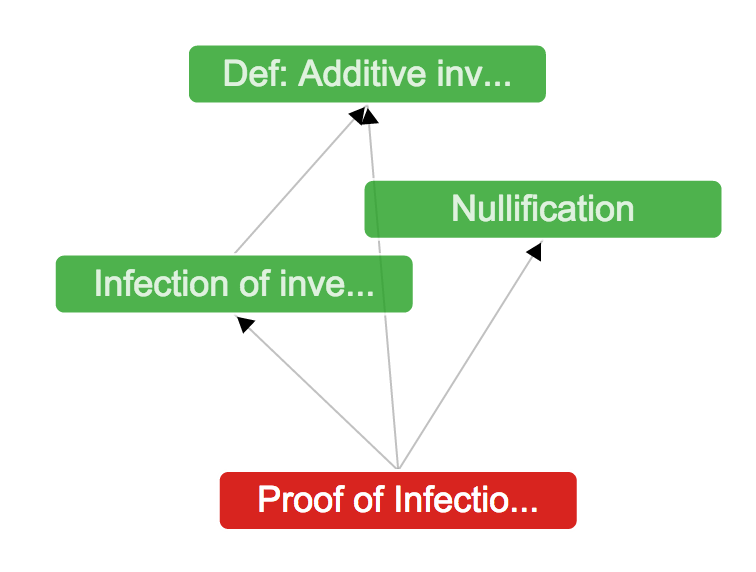
\includegraphics[scale=0.3]{layout_1.png}
\caption{Parent nodes positioned above child nodes (Green: theorem. Red: Proof.)}
\end{figure}
We build the graph layout engine based on D3 Force Layout, which models nodes as repulsing charged particles and edges as elastic cables holding nodes together. The layout algorithm then runs a physics simulation to determine the position of each node.
For each node, we draw a text box with its title inside,
and an arrow from Node $c$ to Node $p$ to indicate that $c$ depends on $p$. Different types of dependencies will be discussed in the next subsection.\\\\
So far the layout engine only takes care of undirected graph structure. 
Ideally, for two nodes $c, p$ with $c$ depending on $p$, we want Node $p$ to stay a little above Node $c$, so that the root of a tree can always be pushed to the top.
In order to do so, we invented our own algorithm.
If our graph is a tree, we can unambiguously compute the height of each node and assign a $y$-coordinate accordingly. 
To deal with cycles, 
we can minimize the potential
\begin{equation}
U(\mathbf{y}) = \sum_{<c,p>}\left(y_p-y_c-H\right)^2,
\end{equation}
where the constant $H$ is vertical spacing per level.
Note that $U(\mathbf{y})\geq0$ and that $U(\mathbf{y})=0$ has solutions if the graph is a tree. 
The solution is not unique because $U(\mathbf{y})$ is invariant under translation of all nodes by the same displacement, 
but this issue turns out to be unimportant.

For example, if we have nodes $1,2,3,4$ with edges 
$(2 \rightarrow 1), (3 \rightarrow 1), (3 \rightarrow 2), (3 \rightarrow 4)$,
the solution (subject to translation) to equation (1)  is

$$y_1=\frac43,~y_2=\frac23,~y_3=0,~y_4=1.$$

We want to use this information to adjust equilibrium positions of nodes in D3 Force Layout,
so we promote minimization of $U(\mathbf{y})$ to a dynamical process,
and a natural choice is gradient descent.
Thus we differentiate $U(\mathbf{y})$ with respect to $y_i$ (and multiply by a constant $-\eta$) to obtain equations of motion 
\begin{equation}
\frac{\mathrm{d}y_i}{\mathrm{d}t} = \eta
\left[
\sum_{<i,p>}\left(y_p-y_i-H\right)
-\sum_{<c,i>}\left(y_i-y_c-H\right)\right],
\end{equation}
which pulls nodes away from their D3 equilibrium positions and minimize the sum of D3 potential and $U(\mathbf{y})$.

\subsubsection{Manipulation}
\begin{figure}[h!]
\centering
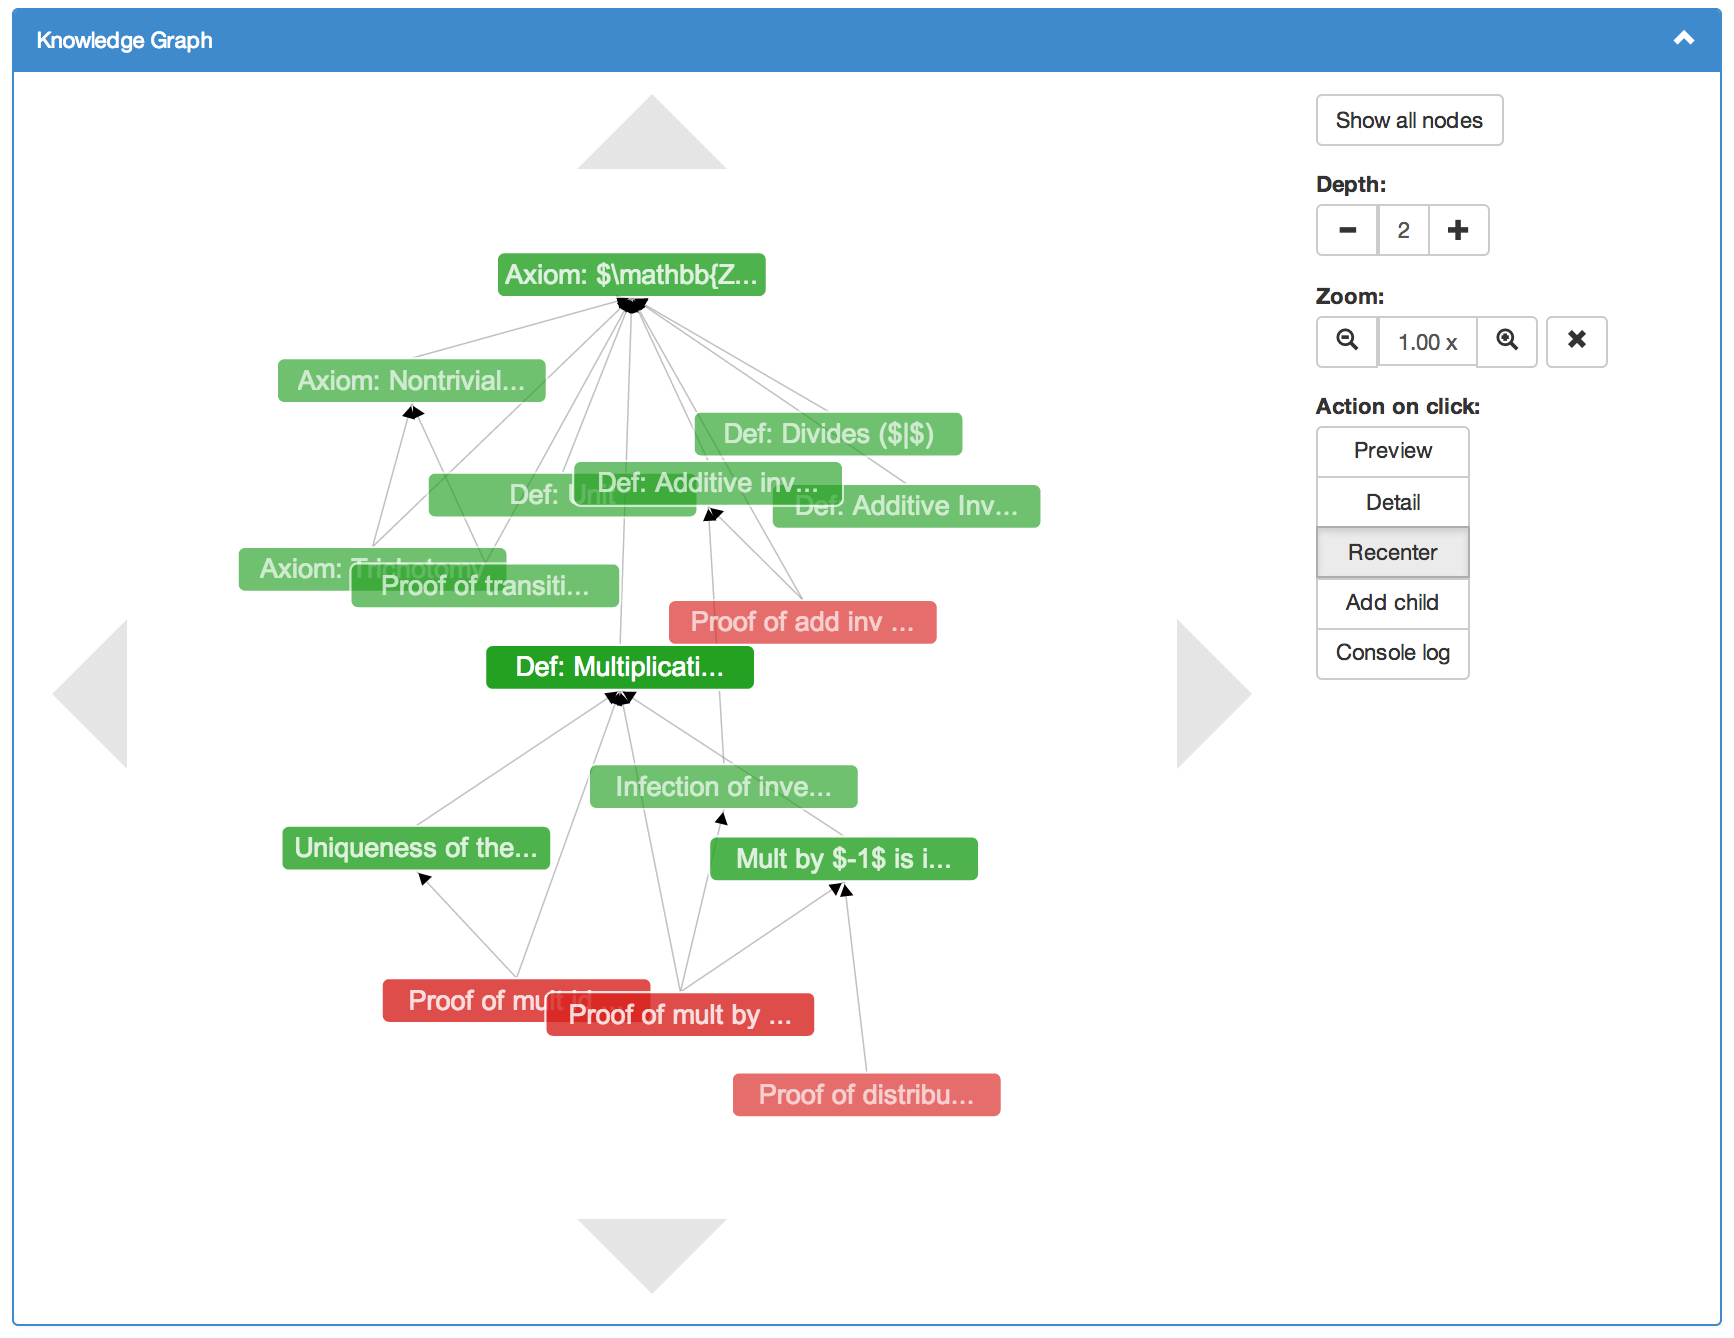
\includegraphics[width=8cm]{toolbar1.png}
\caption{Knowledge graph UI Overview}
\end{figure}

\begin{itemize}
\item Scroll horizontally / vertically
\item Zoom in / zoom out / reset
\item Recenter: change the center node around which the graph is explored
\item Depth: the maximal distance from the center node to display. 
For example, 0 only displays the center node, 1 also displays its parents and children, and 2 also displays its grandparents and grandchildren.
\item Show all nodes: display the whole graph or only nodes around a center node.
\item Preview: open a small window to show the node's content.
\end{itemize}
\begin{figure}[h!]
\centering
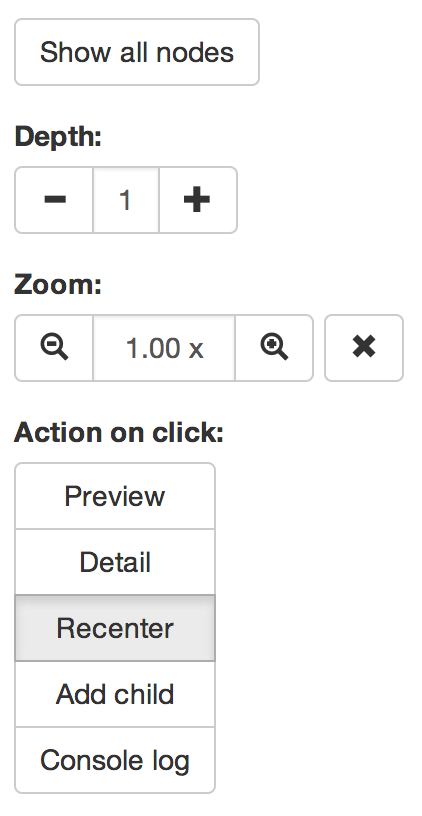
\includegraphics[width=4cm]{toolbar2.png}
\caption{Knowledge graph UI Toolbar}
\end{figure}

\subsection{Web Framework}
The server middleware is based on the Django web-framework. It provides a full set of functionalities for socialmath users to conveniently contribute to the open mathematics library and to build their own knowledge graphs:
\begin{itemize}

\item \emph{Nodes and Dependencies} \\\\
The fundamental functionality in the socialmath web framework is the node-dependency system. In the framework, nodes contain information about its theme, content, type, publication and modification time. We store node-node relationship as well as node-to-other-object relationships. \\
\begin{figure}[h!]
\centering
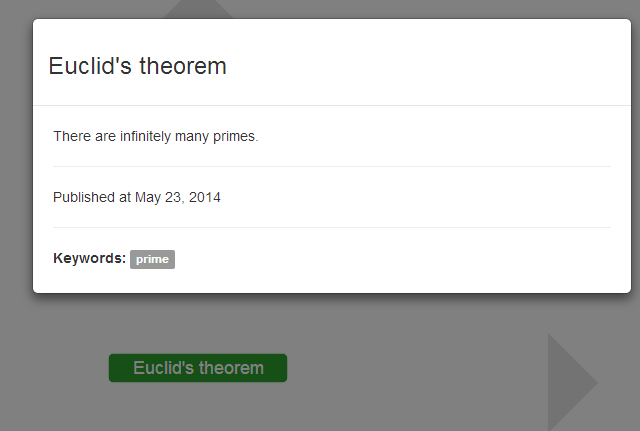
\includegraphics[scale=0.37]{oneNode.png}
\caption{A node in socialmath's knowledge graph}
\end{figure}\\
Dependencies are classified into three types:
\begin{enumerate}
\item \emph{Proof-to-Theorem}: Lemma dependency. This relationship exists when a proof of one theorem cites another theorem in the process. 
\item \emph{Theorem-to-Proof}: Prove dependency. This relationship exists when a proof proves a theorem. 
\begin{figure}[h!]
\centering
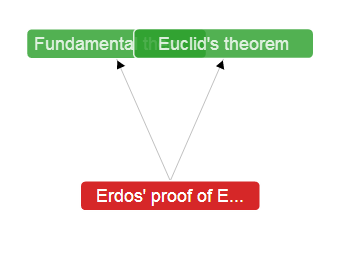
\includegraphics[scale=0.3]{prove_lemma_relationship.png}
\caption{Erd$\tilde{o}$s' proof of Euclid's theorem exhibits prove relationship to Euclid's theorem, and lemma relationship to Fundamental Theorem of Arithmetic}
\end{figure}\
\item \emph{Theorem-to-Theorem}: High-Relevancy dependency. This relationship exists when a theorem is the special case or a generalization of another, or they have strong logical relationship with each other. This also includes the relationship between theorems and definitions. We also model definitions as theorems in our system, except that definitions can't have proofs.
\begin{figure}[h!]
\centering
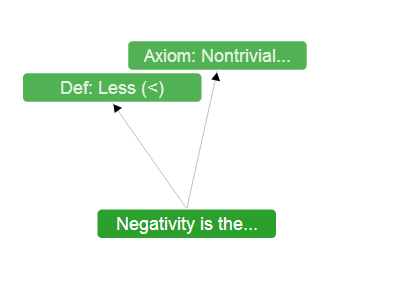
\includegraphics[scale=0.4]{tt_relationship.png}
\caption{Theorem-theorem and theorem-definition relationship}
\end{figure}\
\end{enumerate}

\item \emph{Keywords and Search} \\\\
Keywords are words that imply a node's content and branch of study. They can be added when adding the node, or when editing an existing node. Node-keyword relationships are stored in a relationship set called "Tags". 
The search functionality is supported by keyword mapping. Search can be used in two ways: you can either enter text in the search bar displayed at the index page, or click on the link of an existing keyword. 
\begin{figure}[h!]
\centering
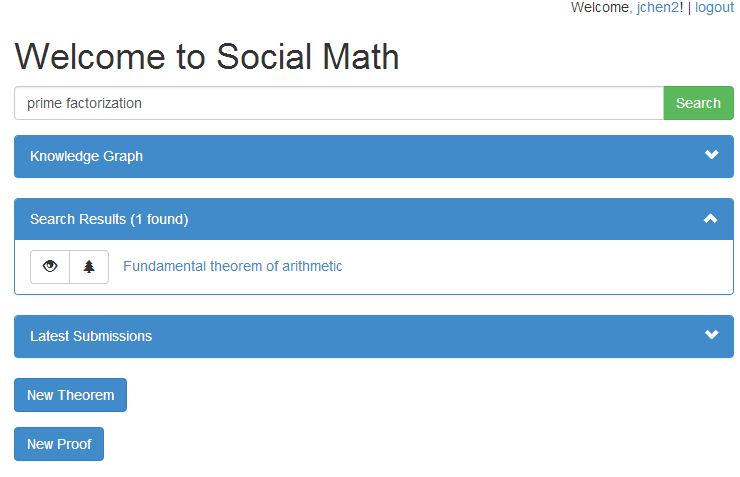
\includegraphics[scale=0.36]{search.png}
\caption{Search results for the keyword "prime factorization"}
\end{figure}\\

\item \emph{Submission and Editing} \\\\
Adding a new theorem or proof can be done in two ways: 
Click on the button at the bottom of the index page, or use the "add child" tool on the graph. \\\\
%\begin{figure}[h!]
%\centering
%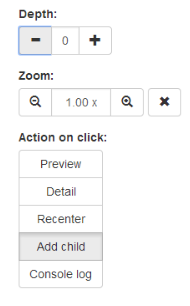
\includegraphics[scale=0.4]{add_child.png}
%\caption{The "add child" tool}
%\end{figure}\\

Users can edit an existing theorem/proof by clicking the "edit" button on the node's detail page. The button links to an interface similar to the add-node page, except that the existing information will be pre populated. 

\item \emph{Users and Profile} \\\\
Socialmath doesn't require a user to login to view its content, but we provide additional functionalities for logged in users. 
Once a user is logged in, his recent activities (adding/editing nodes) will be recorded as events in the database. The events will show up both on the detail page of the modified node, and on the user's profile page. \\
\begin{figure}[h!]
\centering
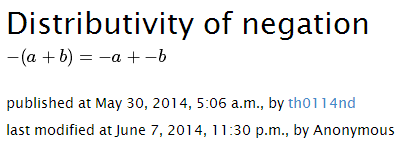
\includegraphics[scale=0.6]{edit_history.png}
\caption{Change history of a node shows the initial author and the last modifier.}
\end{figure}\\
\emph{Follow} is another feature provided for registered users to help keep track of topics they are interested in. The user may click on the "follow" button of any given node, and the server will capture it as a following event. \\
Clicking on a username redirects to that user's profile page. Since there is no search-for-user functionality yet, the only entrance for viewing other users' profiles is through the node's change history. 
\begin{figure}[h!]
\centering
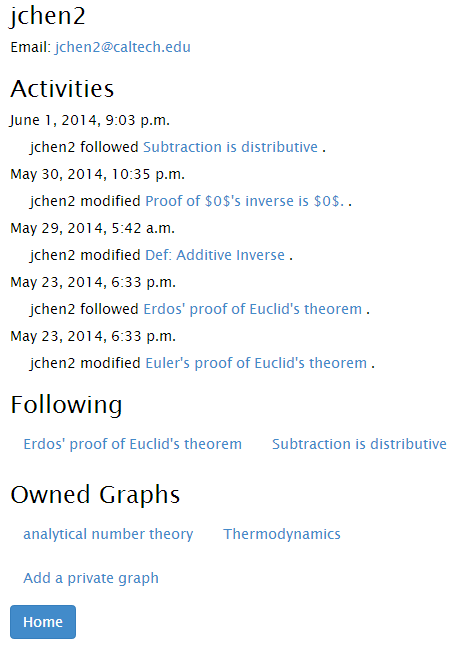
\includegraphics[scale=0.52]{profile.png}
\caption{The profile page of Jianchi Chen, consist of basic info, activities, following-nodes, and private graphs he owns}
\end{figure}\\

\item \emph{Private Graphs} \\\\
In addition to one public knowledge graph visible to everyone, socialmath also provides \emph{private graph} feature so that each registered user can create and edit his own graph. Each private graph has an individual index page. Permission relationship-set makes sure that no nodes in the private graph can be accessed from the public one.   \begin{figure}[h!]
\centering
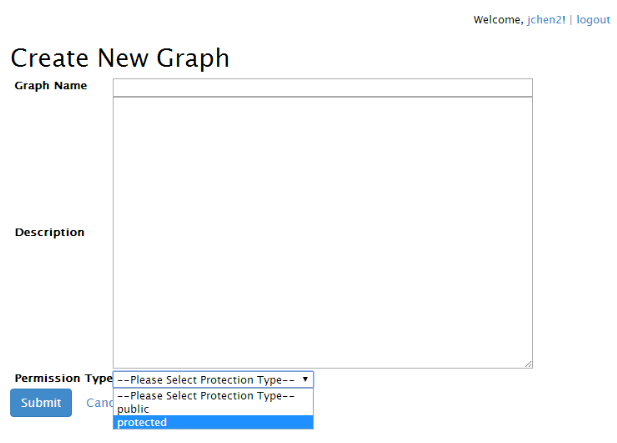
\includegraphics[scale=0.4]{create_pg.png}
\caption{Creating a private graph}
\end{figure}\\
Upon creation, the user may choose to make the graph public or only visible to authorized users. An attempt to view private graph contents when you're not invited will result in a 401 unauthorized error. 
\begin{figure}[h!]
\centering
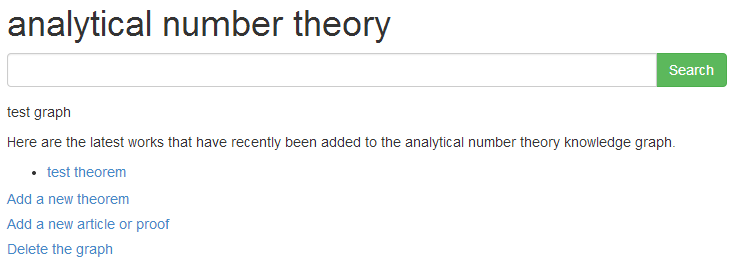
\includegraphics[scale=0.4]{pg_index.png}
\caption{The index page of a private graph, with a node called "test theorem" added.}
\end{figure}\\

\end{itemize}

\subsection{Database}
\subsubsection{Entity-set Schema}
\begin{itemize}
\item Node(\underline{node\_id}, kind, title, statement, pub\_time, last\_modified)
\item Keyword(\underline{kw\_id}, word)
\item PrivateGraph(\underline{pgraph\_id}, name, description, pub\_time, perm\_type)
\item We used the default Django model for user authentication:
User(\underline{user\_id}, username, email, password, ...)\\ 
\end{itemize}

\subsubsection{Relationship-set Schema}
\begin{itemize}
\item Depends(\underline{node\_id}, \underline{node\_id}, dep\_type)
\item Tags(\underline{node\_id}, \underline{kw\_id})
\item Modifies(\underline{node\_id}, \underline{user\_id}, pub\_time, event\_type)
\item Owns(\underline{user\_id}, \underline{pgraph\_id})
\item Includes(\underline{pgraph\_id}, \underline{node\_id})
\end{itemize}

\begin{figure}
\centering
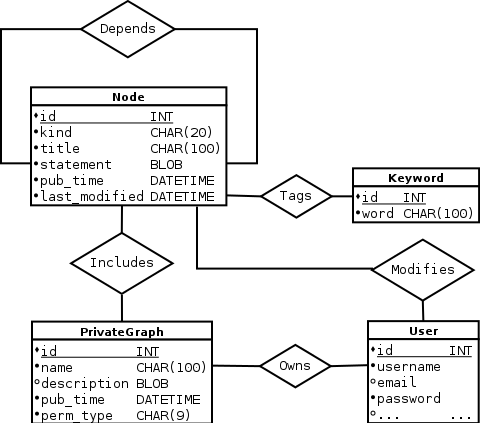
\includegraphics[scale=0.5]{socialmath_ER.png}
\caption{ER Diagram}
\end{figure}


\section{Future Work} 
Here are a few additional 
Although the current socialmath is ready for public usage, there are several additional goals that we plan to achieve with socialmath in the future in order to make it a better product:
\begin{enumerate}
\item \emph{Protection against abuses} \\
Right now, socialmath has no protection against malicious activities such as deleting everything from the knowledge graph, creating dummy nodes, or adding unrelated contents. We can model our protection mechanism after Wikipedia, and build a more comprehensive change history, which allows the system to revert malicious changes and penalize misbehaved users. 
\item \emph{Correctness system} \\
Another concern is that the website currently has no way of assessing the correctness of a proof or a theorem. We can either implement an user upvote system similar to Stack Overflow's, or a user "questioning" system where users can request verification on statements. 
\item \emph{A more collaborative private graph system} \\
An ideal model for a private graph is the github repository. Users are able to collaborate on a graph, fork someone else's work, assign and discuss issues, and use version control. We would also like to include visualization in the private graph. 
\item \emph{File support} \\
In addition to in-box writing, we should support pdf upload and display, so that users can also make contributions by finding existing write ups. 
\item \emph{Lemma and keyword detection} \\
A more advanced version of the socialmath node submission system includes lemma and keyword auto-detection. A simple algorithm is to collect statistics on the text's N-grams (sequences of $n$ consecutive words).  Sequences with a significant number of occurrences are then candidates for the keyword/lemma \cite{Kumar:2008:AKE:1410140.1410180}.
\item \emph{Better user interaction} \\
There's a lot of room for enhancing the "social" side of the current product. The first step is to implement handy features such as user searching, following, and in-site messaging. We can implement a level-based experience system to reward active and reliable users. We should also reward users who manage to invite new users.
\end{enumerate}

%ACKNOWLEDGMENTS are optional
\section{Acknowledgments}
We would like to thank our faculty advisor, Professor Steven
Low, and our teaching assistant, Qiuyu Peng, for their feedback and guidance.We would also like to thank Professor Adam Wierman for co-hosting the class.

%
% The following two commands are all you need in the
% initial runs of your .tex file to
% produce the bibliography for the citations in your paper.
\bibliographystyle{plain}
\bibliography{socialmath} 
% You must have a proper ".bib" file
%  and remember to run:
% latex bibtex latex latex
% to resolve all references
%
% ACM needs 'a single self-contained file'!
%
%APPENDICES are optional
%\balancecolumns

% That's all folks!

\end{document}
